% http://home.agh.edu.pl/~vlsi/AI/backp_t_en/backprop.html
%\ifx\du\undefined
%  \newlength{\du}
%\fi
%\newcommand{\nweigth}[2]{$W^{#1}_{#2} - \alpha\frac{\partial J}{\partial W^{#1}_{#2}}$}
%\newcommand{\w}[2]{$W^{#1}_{#2}$}

%\setlength{\du}{15\unitlength}
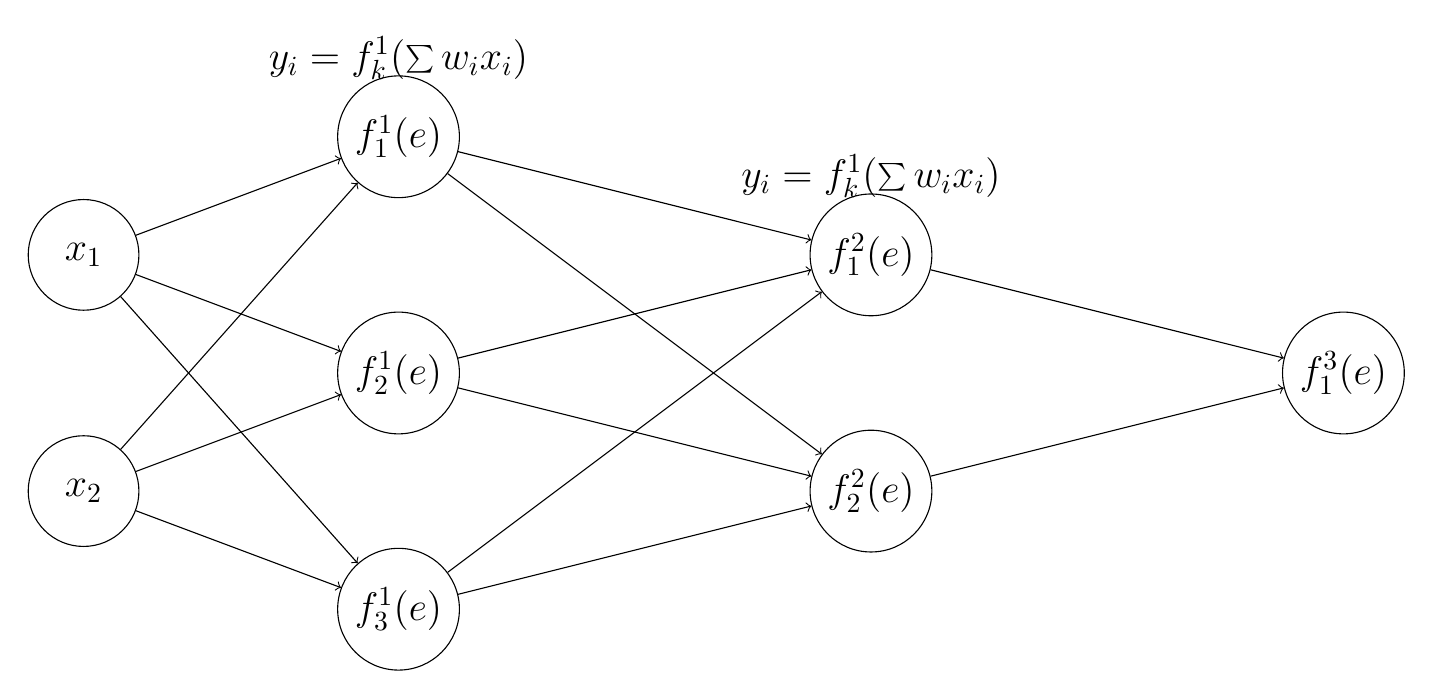
\begin{tikzpicture}
\tikzstyle{neuron}=[circle,draw, minimum size=4em, font=\Large]
\tikzstyle{update}=[dashed, blue]

\coordinate (x_1) at (-5, 1.5);
\coordinate (x_2) at (-5, -1.5);

\coordinate (n_1_1) at (-1, 3);
\coordinate (n_1_2) at (-1, 0);
\coordinate (n_1_3) at (-1, -3);

\coordinate (n_2_1) at (5, 1.5);
\coordinate (n_2_2) at (5, -1.5);

\coordinate (n_3_1) at (11, 0);


\node[neuron] (x_1) at (x_1) {$x_{1}$};
\node[neuron] (x_2) at (x_2) {$x_{2}$};

\node[neuron] (n_1_1) at (n_1_1) {$f^{1}_{1}(e)$};
\node[neuron] (n_1_2) at (n_1_2) {$f^{1}_{2}(e)$};
\node[neuron] (n_1_3) at (n_1_3) {$f^{1}_{3}(e)$};

\node[neuron] (n_2_1) at (n_2_1) {$f^{2}_{1}(e)$};
\node[neuron] (n_2_2) at (n_2_2) {$f^{2}_{2}(e)$};

\node[neuron] (n_3_1) at (n_3_1) {$f^{3}_{1}(e)$};


\node[above of=n_1_1] {\Large $y_i = f^{1}_{k}(\sum w_i x_i)$};
\node[above of=n_2_1] {\Large $y_i = f^{1}_{k}(\sum w_i x_i)$};
%\node[above of=n_3_1] {\Large $y_i = f^{1}_{k}(\sum w_i x_i)$};

\draw[->] (x_1) -- (n_1_1);
\draw[->] (x_1) -- (n_1_2);
\draw[->] (x_1) -- (n_1_3);
\draw[->] (x_2) -- (n_1_1);
\draw[->] (x_2) -- (n_1_2);
\draw[->] (x_2) -- (n_1_3);

\draw[->] (n_1_1) -- (n_2_1);
\draw[->] (n_1_1) -- (n_2_2);
\draw[->] (n_1_2) -- (n_2_1);
\draw[->] (n_1_2) -- (n_2_2);
\draw[->] (n_1_3) -- (n_2_1);
\draw[->] (n_1_3) -- (n_2_2);

\draw[->] (n_2_1) -- (n_3_1);
\draw[->] (n_2_2) -- (n_3_1);

\end{tikzpicture}
